\documentclass[11pt,a4paper]{article}
\usepackage[utf8]{inputenc}
\usepackage[T1]{fontenc}
\IfFileExists{french.ldf}{\usepackage[french]{babel}}{\usepackage[english]{babel}}
\usepackage{amsmath,amssymb,amsthm}
\usepackage{geometry}\geometry{margin=2.4cm}
\usepackage{listings}
\usepackage{xcolor}
\usepackage{enumitem}
\usepackage{lmodern}
\usepackage{tikz}
\usepackage{hyperref}
\hypersetup{colorlinks=true, urlcolor=[RGB]{2,101,115}, linkcolor=black, citecolor=black}
\definecolor{codebg}{RGB}{247,249,251}
\definecolor{kw}{RGB}{175,45,45}
\definecolor{cmt}{RGB}{110,120,130}
\definecolor{str}{RGB}{20,110,60}
\lstset{language=Python, backgroundcolor=\color{codebg}, basicstyle=\ttfamily\small,
  keywordstyle=\color{kw}\bfseries, commentstyle=\color{cmt}\itshape, stringstyle=\color{str},
  numbers=left, numberstyle=\tiny\color{cmt}, numbersep=8pt, frame=single, rulecolor=\color{gray!40},
  showstringspaces=false, breaklines=true, columns=fullflexible, extendedchars=true, inputencoding=utf8,
  literate={é}{{\'e}}1 {è}{{\`e}}1 {à}{{\`a}}1 {ê}{{\^e}}1 {î}{{\^i}}1 {ç}{{\c c}}1 {ô}{{\^o}}1 {û}{{\^u}}1 {ù}{{\`u}}1 {É}{{\'E}}1}
\newcommand{\code}[1]{\lstinline!#1!}
\theoremstyle{definition}\newtheorem{definition}{Définition}
\theoremstyle{plain}\newtheorem{theoreme}{Théorème}\newtheorem{proposition}{Proposition}\newtheorem{lemme}{Lemme}
\theoremstyle{remark}\newtheorem{remarque}{Remarque}
\renewcommand{\proofname}{Démonstration}
\setlength{\parskip}{0.35em}

\begin{document}

\begin{center}
{\large\bfseries Agrégation externe de mathématiques}\\[3pt]
{\bfseries Épreuve de modélisation --- Option C : algèbre et calcul formel}\\[10pt]
\rule{0.85\linewidth}{0.4pt}\\[8pt]
{\LARGE\bfseries Structures de données authentifiées :\\[2pt] arbres de Merkle et preuves d'inclusion}\\[8pt]
\rule{0.85\linewidth}{0.4pt}
\end{center}

\medskip
\begin{center}
\fbox{\begin{minipage}{0.95\linewidth}\small
Il est rappelé que le jury n'exige pas une compréhension exhaustive du texte. Vous êtes
laissé(e) libre d'organiser votre présentation comme vous l'entendez. Il vous est conseillé de
mettre en valeur vos connaissances et votre culture scientifique à partir du fil conducteur
constitué par le texte. Les \emph{suggestions de développement}, en fin de texte, ne sont là que
pour vous aider~; vous ne devez pas vous sentir tenu(e) de les suivre, ni de les traiter toutes.
Le jury appréciera que votre exposé soit accompagné d'\textbf{exemples et d'expériences traités
sur ordinateur}.
\end{minipage}}
\end{center}

\bigskip
\section{Un problème de vérification à faible coût}

Les registres distribués (\emph{blockchains}) comme Bitcoin ou Ethereum maintiennent, sur des
milliers de machines indépendantes, un état commun de très grande taille. Une opération y revient
sans cesse~: \emph{convaincre} un participant qu'une donnée précise (une transaction, un solde,
une adresse figurant sur une liste d'autorisation) appartient bien à un ensemble donné, \emph{sans}
lui transmettre l'ensemble entier ni exiger qu'il le recalcule. Le coût de stockage et de
communication \guillemotleft~sur la chaîne~\guillemotright{} étant élevé, on cherche des
\emph{certificats} de taille aussi petite que possible.

Formulons le problème. On dispose d'une suite finie de données $d_0, d_1, \dots, d_{n-1}$ (les
\emph{feuilles}). Un acteur, le \emph{prouveur}, publie un unique condensé $R$ résumant toute la
suite. Plus tard, il veut prouver à un \emph{vérifieur} que \guillemotleft~$d_i$ figure à la
position $i$ dans la suite ayant produit $R$~\guillemotright, en fournissant un certificat de
taille minimale. Le vérifieur ne connaît que $R$ et la donnée $d_i$ présentée~; il doit pouvoir
\emph{rejeter} toute donnée qui ne figurait pas réellement dans la suite.

L'objet de ce texte est la solution devenue standard, l'\emph{arbre de Merkle} (R.~Merkle, 1979),
qui atteint des certificats de taille $O(\log n)$. Elle repose entièrement sur une brique
cryptographique, la \emph{fonction de hachage résistante aux collisions}, que nous étudions
d'abord. Le fil conducteur mêle arithmétique modulaire, dénombrement, un argument probabiliste
(le \emph{paradoxe des anniversaires}) et une preuve de correction par récurrence.

\section{Fonctions de hachage et résistance aux collisions}

\begin{definition}
Une \emph{fonction de hachage} est une application $H : \mathcal{M} \to \{0,1,\dots,M-1\}$ d'un
ensemble de messages $\mathcal{M}$ (potentiellement infini) vers un ensemble fini de $M$ valeurs.
Une \emph{collision} est un couple de messages distincts $m \neq m'$ tels que $H(m) = H(m')$.
\end{definition}

Dans les implémentations réelles on prend $M = 2^{b}$ (par exemple $b = 256$ pour Keccak-256,
utilisée par Ethereum). Pour les besoins des \emph{expériences}, on pourra travailler avec la
fonction de combinaison arithmétique jouet
\begin{equation}\label{eq:parent}
  h(a,b) = (31\,a + b) \bmod p, \qquad p = 1000003 \ \text{premier},
\end{equation}
qui joue le rôle d'un \guillemotleft~hachage de deux valeurs en une~\guillemotright.

L'observation fondamentale est que les collisions \emph{existent} nécessairement.

\begin{proposition}[Principe des tiroirs]\label{prop:tiroirs}
Si $\mathcal{M}$ est de cardinal strictement supérieur à $M$ (en particulier s'il est infini),
alors $H$ n'est pas injective~: elle admet au moins une collision.
\end{proposition}

\begin{proof}
Si $H$ était injective, elle réaliserait une bijection de $\mathcal{M}$ sur une partie de
l'ensemble d'arrivée, de cardinal au plus $M$~; on aurait $|\mathcal{M}| \le M$, ce qui contredit
l'hypothèse. Il existe donc $m \neq m'$ avec $H(m) = H(m')$.
\end{proof}

La sécurité ne peut donc pas reposer sur l'\emph{absence} de collisions. On demande seulement
qu'elles soient \emph{calculatoirement introuvables}.

\begin{definition}
$H$ est dite \emph{résistante aux collisions} s'il n'existe pas d'algorithme efficace (en temps
polynomial) produisant, avec probabilité non négligeable, une collision de $H$.
\end{definition}

C'est une hypothèse \emph{cryptographique}, non un théorème~: elle porte sur la difficulté
algorithmique, pas sur l'inexistence. Quantifions la difficulté de trouver une collision par
\emph{recherche aveugle}, en modélisant $H$ comme un tirage uniforme dans $\{0,\dots,M-1\}$
(modèle de l'\emph{oracle aléatoire}).

\begin{proposition}[Borne des anniversaires]\label{prop:birthday}
On tire $k$ valeurs indépendantes et uniformes dans un ensemble à $M$ éléments. La probabilité
$q_k$ qu'elles soient \emph{deux à deux distinctes} vaut
\[
  q_k = \prod_{i=0}^{k-1}\Bigl(1 - \frac{i}{M}\Bigr),
  \qquad\text{et}\qquad
  q_k \le \exp\!\Bigl(-\frac{k(k-1)}{2M}\Bigr).
\]
En particulier, la probabilité d'au moins une collision dépasse $1/2$ dès que
$k \gtrsim 1{,}177\,\sqrt{M}$.
\end{proposition}

\begin{proof}
Le $i$-ième tirage évite les $i$ valeurs déjà obtenues avec probabilité $1 - i/M$~; par
indépendance, $q_k$ est le produit annoncé. En utilisant $1 - x \le e^{-x}$ pour tout $x$, on
majore $q_k \le \prod_{i=0}^{k-1} e^{-i/M} = \exp\!\bigl(-\tfrac{1}{M}\sum_{i=0}^{k-1} i\bigr)
= \exp\!\bigl(-\tfrac{k(k-1)}{2M}\bigr)$. La probabilité de collision $1 - q_k$ dépasse $1/2$
lorsque $q_k \le 1/2$, ce qui est assuré dès que $\tfrac{k(k-1)}{2M} \ge \ln 2$, soit
$k \gtrsim \sqrt{2\ln 2}\,\sqrt{M} \approx 1{,}177\,\sqrt{M}$.
\end{proof}

Ainsi une fonction sur $b$ bits n'offre qu'une sécurité de l'ordre de $2^{b/2}$ opérations contre
les collisions~: c'est pourquoi on choisit $b = 256$ (soit $\approx 2^{128}$, hors de portée).
Le cas familier $M = 365$ redonne le \emph{paradoxe des anniversaires}~: $23$ personnes suffisent
à rendre une coïncidence plus probable qu'improbable. On pourra vérifier ces seuils par une
\textbf{simulation de Monte-Carlo}~:

\begin{lstlisting}
import random
def collision_probable(M, k, essais=20000):
    succes = 0
    for _ in range(essais):
        vus = set(); coll = False
        for _ in range(k):
            v = random.randrange(M)
            if v in vus: coll = True; break
            vus.add(v)
        succes += coll
    return succes / essais
# collision_probable(365, 23)   ~ 0.50
# collision_probable(10**6, 1178) ~ 0.50
\end{lstlisting}

\section{Arbres de Merkle}

L'idée est de \emph{hacher par niveaux}. Les feuilles $d_0, \dots, d_{n-1}$ (déjà hachées, vues
comme des entiers) forment le niveau $0$~; on remplace chaque paire consécutive par son haché
combiné $h(\cdot,\cdot)$, obtenant le niveau $1$, deux fois plus court~; on itère jusqu'à ne
conserver qu'une valeur, la \emph{racine} $R$. Lorsqu'un niveau a une longueur impaire, on
\emph{duplique} sa dernière valeur avant l'appariement.

\begin{center}
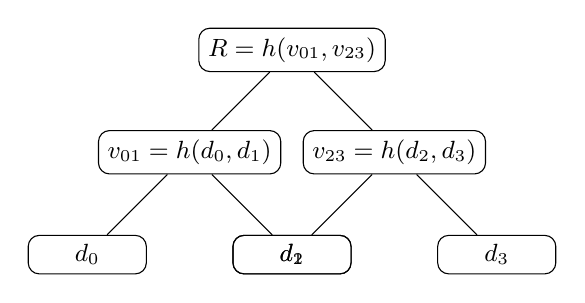
\begin{tikzpicture}[level distance=13mm, sibling distance=26mm,
  every node/.style={draw, rounded corners, minimum width=15mm, font=\small}]
\node {$R=h(v_{01},v_{23})$}
  child {node {$v_{01}=h(d_0,d_1)$}
    child {node {$d_0$}}
    child {node {$d_1$}}}
  child {node {$v_{23}=h(d_2,d_3)$}
    child {node {$d_2$}}
    child {node {$d_3$}}};
\end{tikzpicture}
\end{center}
\begin{center}\small Figure~1 --- Arbre de Merkle sur quatre feuilles.\end{center}

Avec la fonction jouet~\eqref{eq:parent} et les feuilles $[1,2,3,4]$ on obtient
$v_{01}=h(1,2)=33$, $v_{23}=h(3,4)=97$, puis $R=h(33,97)=1120$. Voici la construction~:

\begin{lstlisting}
def h(a, b):
    return (31 * a + b) % 1000003

def racine(feuilles):
    niveau = list(feuilles)
    while len(niveau) > 1:
        if len(niveau) % 2 == 1:
            niveau.append(niveau[-1])          # duplication si impair
        niveau = [h(niveau[i], niveau[i+1])
                  for i in range(0, len(niveau), 2)]
    return niveau[0]
# racine([1, 2, 3, 4]) == 1120
\end{lstlisting}

\begin{proposition}[Complexité]\label{prop:complexite}
Le calcul de la racine de $n$ feuilles effectue $O(n)$ évaluations de $h$, en temps $O(n)$ et
espace $O(n)$. L'arbre a une hauteur $H(n) = \lceil \log_2 n \rceil$.
\end{proposition}

\begin{proof}
Notons $t_0 = n$ et $t_{k+1} = \lceil t_k/2 \rceil$ la taille du niveau $k+1$~; ce niveau demande
$\lceil t_k / 2 \rceil$ évaluations de $h$. Comme $t_{k+1} \le t_k/2 + 1$, une récurrence donne
$t_k \le n\,2^{-k} + 2$, donc $t_k \le 2$ dès que $k \ge \log_2 n$~: la hauteur est
$\lceil \log_2 n\rceil$ et il y a $O(\log n)$ niveaux. Le nombre total d'évaluations vaut
$\sum_{k \ge 1} t_k \le \sum_{k\ge 1}\bigl(n\,2^{-k} + 2\bigr) \le n + O(\log n) = O(n)$.
\end{proof}

\section{Preuves d'inclusion et sécurité}

\begin{definition}
Une \emph{preuve d'inclusion} de la feuille d'indice $i$ est la suite des couples
$(\text{fr\`ere}, \text{côté})$ rencontrés en remontant de cette feuille jusqu'à la racine, où le
côté indique si le frère se situe à gauche (\texttt{L}) ou à droite (\texttt{R}). Pour la
vérifier, on repart de la feuille présentée et l'on recombine successivement par $h$ avec chaque
frère selon son côté~; la feuille est \emph{acceptée} si l'on retrouve la racine $R$.
\end{definition}

Sur la Figure~1, la preuve de $d_0$ est $\bigl[(d_1,\texttt{R}),(v_{23},\texttt{R})\bigr]$~: le
vérifieur calcule $h(d_0, d_1) = v_{01}$ puis $h(v_{01}, v_{23}) = R$. La longueur d'une preuve
est le nombre de niveaux, soit $H(n) = \lceil \log_2 n\rceil = O(\log n)$~: pour un milliard de
feuilles, une trentaine de valeurs suffisent, à comparer à la transmission des $n$ feuilles. C'est
tout l'intérêt de la construction.

Reste la propriété de sécurité~: un prouveur malhonnête ne doit pas pouvoir faire accepter une
feuille absente. C'est ici que sert l'hypothèse de résistance aux collisions.

\begin{theoreme}[Correction, ou \emph{soundness}]\label{th:soundness}
Supposons $h$ résistante aux collisions. Si la vérification d'une preuve d'inclusion pour une
valeur $x$ aboutit à la racine authentique $R$, alors, sauf à exhiber une collision de $h$, la
valeur $x$ figure effectivement parmi les feuilles ayant produit $R$.
\end{theoreme}

\begin{proof}
Récurrence sur la hauteur $H$ de l'arbre. Si $H = 0$, l'arbre est réduit à sa racine, qui
\emph{est} la feuille~; la preuve est vide et n'est acceptée que si $x = R$, donc $x$ est bien la
feuille. Supposons le résultat acquis à la hauteur $H$ et considérons un arbre de hauteur $H+1$,
de racine $R = h(g, d)$ où $g, d$ sont les deux valeurs de niveau $1$ réellement présentes. La
vérification calcule d'abord $r' = h(x, f)$ (ou $h(f, x)$) avec le premier frère $f$, puis
poursuit avec le reste de la preuve~: c'est une vérification d'inclusion de $r'$ dans l'arbre des
n\oe uds de niveau $1$, de hauteur $H$. Par hypothèse de récurrence, ou bien $r'$ est l'un des
n\oe uds authentiques de ce niveau, ou bien on a exhibé une collision. Dans le premier cas,
$r' \in \{g, d\}$ et $r' = h(x, f)$~; comme $r'$ possède déjà l'antécédent authentique issu de la
construction, l'égalité $h(x,f) = r'$ fournit soit \emph{le même} couple (et alors $x$ est la
feuille voulue), soit un couple \emph{différent} de même image, c'est-à-dire une collision de $h$.
En l'absence de collision calculable, $x$ figure donc bien parmi les feuilles.
\end{proof}

\begin{remarque}
La sécurité de tout l'édifice se \emph{réduit} ainsi à celle de $h$~: forger une fausse preuve
d'inclusion, c'est calculer une collision. Cette \emph{réduction} est l'exacte raison pour
laquelle on exige $b = 256$ bits (Proposition~\ref{prop:birthday}).
\end{remarque}

\section{Aspects dynamiques et prolongements}

\paragraph{Mises à jour.} Lorsqu'une seule feuille change, seuls les n\oe uds situés sur le
chemin de cette feuille à la racine sont affectés~: il y en a $H(n) = O(\log n)$. En conservant
les n\oe uds inchangés, une mise à jour de la racine ne coûte donc que $O(\log n)$ évaluations de
$h$, et non $O(n)$. Cette propriété est essentielle pour les \guillemotleft~arbres de Merkle
persistants~\guillemotright{} qui indexent l'état d'Ethereum.

\paragraph{Au-delà.} Les arbres de Merkle sont un cas particulier d'\emph{accumulateur
cryptographique}. Ethereum emploie une variante, l'arbre de \emph{Patricia-Merkle}, mêlant arbre
préfixe et hachage~; le projet \emph{Verkle} remplace le hachage binaire par des \emph{engagements
polynomiaux} (schémas de type KZG) afin de réduire encore la taille des preuves, de $O(\log n)$ à
$O(1)$. Enfin, la vérification \guillemotleft~à faible coût~\guillemotright{} illustrée ici est
l'idée directrice des \emph{preuves à divulgation nulle de connaissance} et des \emph{rollups}~:
faire vérifier un calcul massif à moindre frais.

\section*{Suggestions pour le développement}

\emph{Les pistes suivantes sont largement indépendantes~; on n'en traitera qu'une partie.}

\begin{itemize}[nosep,leftmargin=1.3em]
  \item Démontrer soigneusement la Proposition~\ref{prop:birthday} et discuter l'équivalent
        asymptotique du seuil $k^\star(M)$~; comparer aux mesures de la simulation de Monte-Carlo
        (cas $M=365$, $M=10^6$, $M=2^{32}$).
  \item Implémenter la construction de l'arbre, la génération et la vérification des preuves
        d'inclusion~; mesurer expérimentalement la taille des preuves en fonction de $n$ et
        confronter à $\lceil\log_2 n\rceil$.
  \item Détailler la preuve du Théorème~\ref{th:soundness} et expliciter la
        \emph{réduction}~: comment une fausse preuve fournit-elle algorithmiquement une collision~?
  \item Étudier le coût amorti des mises à jour dynamiques~; programmer une version en
        $O(\log n)$ conservant les n\oe uds inchangés et la comparer au recalcul complet.
  \item Analyser l'arithmétique de la fonction jouet~\eqref{eq:parent}~: pour quels choix de
        multiplicateur et de module $p$ obtient-on une bonne dispersion~? Relier au hachage
        polynomial et aux corps $\mathbb{Z}/p\mathbb{Z}$.
  \item Comparer, en taille de preuve et en coût de vérification, l'arbre de Merkle binaire, un
        arbre $k$-aire, et un engagement vectoriel de type Verkle.
  \item Modéliser une \emph{liste d'autorisation} (\emph{whitelist}) d'adresses par sa racine de
        Merkle~; estimer l'économie de stockage \guillemotleft~sur la chaîne~\guillemotright.
  \item Situer le problème de sécurité dans le cadre des \emph{fonctions à sens unique} et des
        hypothèses de la cryptographie moderne.
\end{itemize}

\section*{Références}

\begin{enumerate}[nosep,leftmargin=1.6em]
  \item R.~C.~Merkle, \emph{A digital signature based on a conventional encryption function},
        CRYPTO~'87.
  \item A.~M.~Antonopoulos, G.~Wood, \emph{Mastering Ethereum}, O'Reilly, 2\textsuperscript{e}~éd.
        (chapitres \guillemotleft~Cryptography~\guillemotright, \guillemotleft~The Ethereum Virtual
        Machine~\guillemotright, \guillemotleft~Decentralized Applications~\guillemotright).
  \item J.~Katz, Y.~Lindell, \emph{Introduction to Modern Cryptography}, CRC Press.
  \item D.~Boneh, V.~Shoup, \emph{A Graduate Course in Applied Cryptography} (chapitre sur les
        fonctions de hachage et la borne des anniversaires).
\end{enumerate}

\vfill
\noindent\rule{\linewidth}{0.3pt}\\
{\footnotesize\itshape Texte proposé dans le cadre d'une préparation à l'agrégation par
Pr Agrégé El Hadiq Zouhair --- \href{https://cpgeacademy.org}{cpgeacademy.org}. Toutes les valeurs
numériques et les fonctions ont été vérifiées par ordinateur.}

\end{document}
